\documentclass{book}

\usepackage[a4paper]{geometry}

\usepackage[T2A]{fontenc}
\usepackage[utf8]{inputenc}
\usepackage[english,russian]{babel}

\usepackage{graphicx}

\begin{document}

\tableofcontents

\part{Описание конструктора}

\chapter{Релейная логика}

\part{Лабораторные работы}

\chapter{Калькулятор}

\section{Тумблеры}

Модуль с тумблерами используется для ручного включения и выключения реле.
Присоединяя его к разным разъёмам, можно задавать четырёхбитное число,
либо переключать до четырёх управляющих сигналов.

Проще всего проверить работу тумблеров, подключив их к управляющей шине
регистрового модуля, в который вставлены только $4$ реле.

\subsection{Практикум}

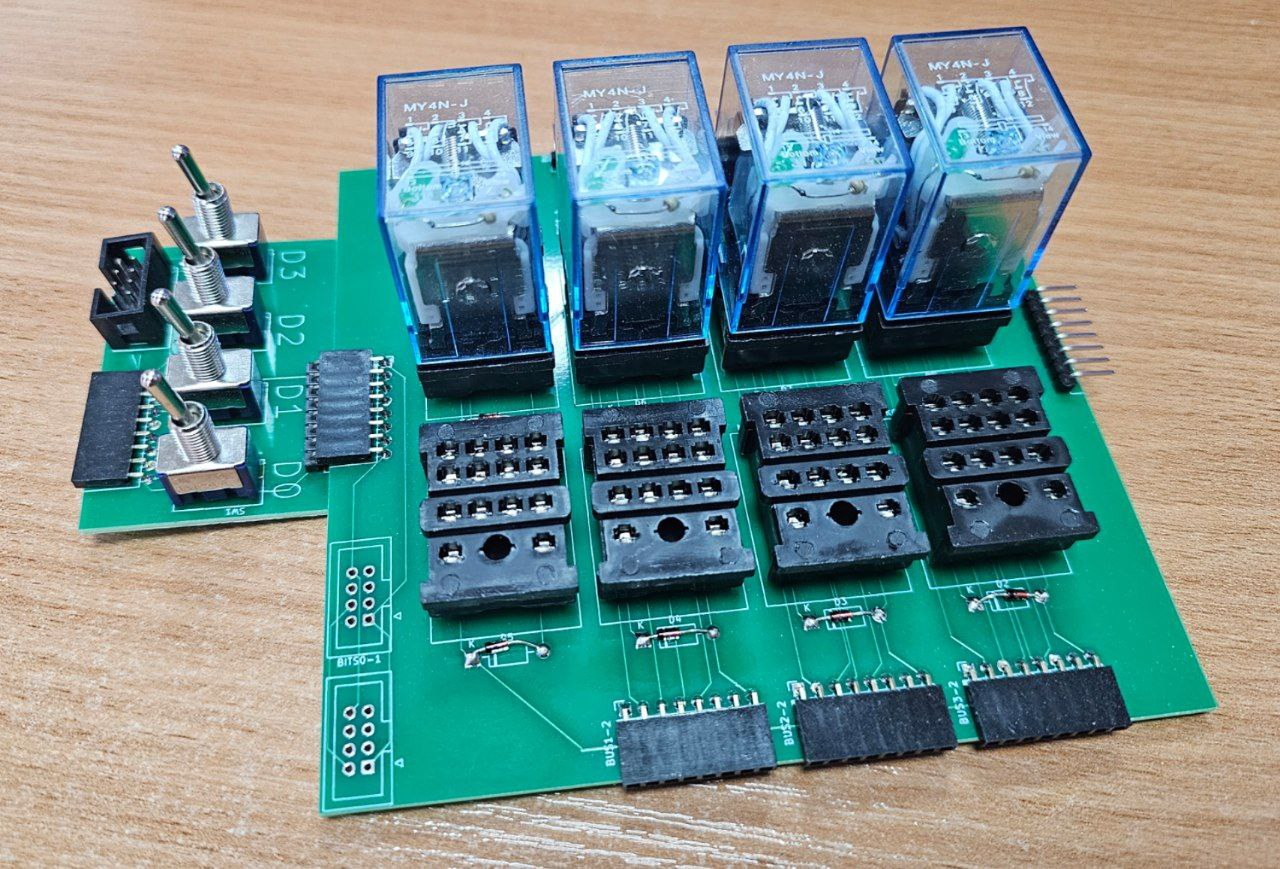
\includegraphics[width=0.5\columnwidth]{photo/switches.jpg}

\begin{enumerate}
    \item Переключать тумблеры. Убедиться, что положение одного тумблера меняет состояние одного реле.
    \item Запомнить включенное и выключенное состояния тумблера, чтобы позднее не было проблем с управлением другими схемами.
\end{enumerate}

\section{Регистр}

Модуль четырёхбитного регистра состоит из четырёх реле-триггеров,
одного реле для обнуления регистра и трёх реле для подключения
к шинам данных.

Модуль <<Регистр>> имеет следующие разъёмы:
\begin{itemize}
  \item Слева и справа: управляющие сигналы сброса и выборки.
        Можно подключить тумблеры
        для ручного включения сигналов. Также можно соединить несколько
        модулей регистра, чтобы управлять одним набором сигналов сразу
        для $8$, $12$ \ldots бит.
  \item Сверху и снизу: три шины данных. Реле регистра могут
        подключаться к шинам для записи или чтения данных.
  \item Дополнительные разъёмы с битами $0-3$ и $2-3$ для чтения или
        записи значения без подключения к шине.
\end{itemize}

\subsection{Практикум}

Протестировать работу регистра можно собрав следующую схему:

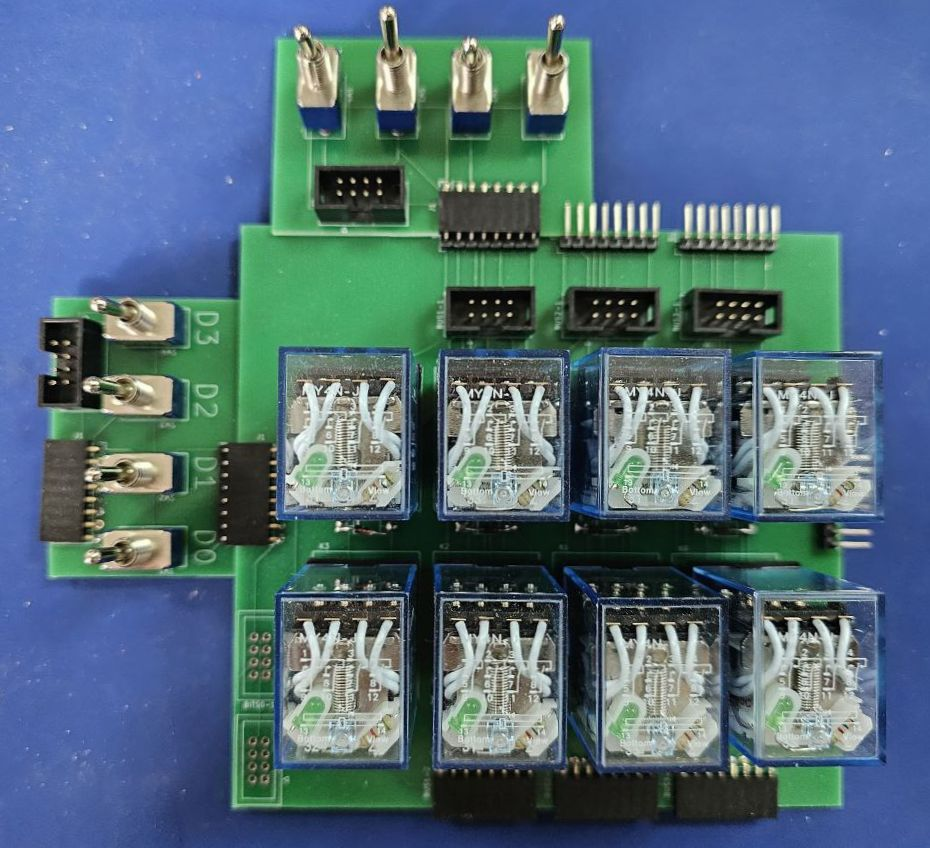
\includegraphics[width=0.5\columnwidth]{photo/register.jpg}

\begin{itemize}
  \item Тумблеры слева управляют работой регистра. Бит 0 --- обнуление, бит 1 --- выборка на шину 1.
  \item Тумблеры сверху нужны для ввода значения регистра. Когда он подключается к шине 1,
        значения, набранное на тумблерах, записывается в регистр.
\end{itemize}

\subsubsection{Регистр без шины}

\begin{enumerate}
    \item Подключить тубмлеры проводом к битам $0-3$ вместо шины.
    \item Набирать значение, убедиться, что биты переключаются в $1$, но не возвращаются в $0$.
    \item Обнулить тумблеры с данными.
    \item Включить и выключить сигнал сброса. Убедиться, что значения всех битов теперь $0$.
\end{enumerate}

\subsubsection{Регистр с шиной}

\begin{enumerate}
    \item Отключить все управляющие сигналы.
    \item Набрать значение на тумблерах для данных. Убедиться, что это не влияет на регистр.
    \item Включить и выключить сигнал выборки на шину $1$. Убедиться, что данные записались в регистр.
    \item Включить и выключить сигнал сброса. Убедиться, что значения всех битов теперь $0$.
\end{enumerate}

\section{Шина и регистровый файл}

Несколько регистров можно соединить в регистровый файл.
У каждого из регистров есть сигналы выборки на одну из трёх шин.

Если два регистра подключены к одной шине одновременно,
то значения одного будут копироваться в другой. Если точнее,
включённые биты включают аналогичные в другом регистре, то есть
копирование возможно в обе стороны одновременно.

Нулевые биты при этом копироваться не могут. Для записи нулей
регистр необходимо сбросить.


\subsection{Практикум}


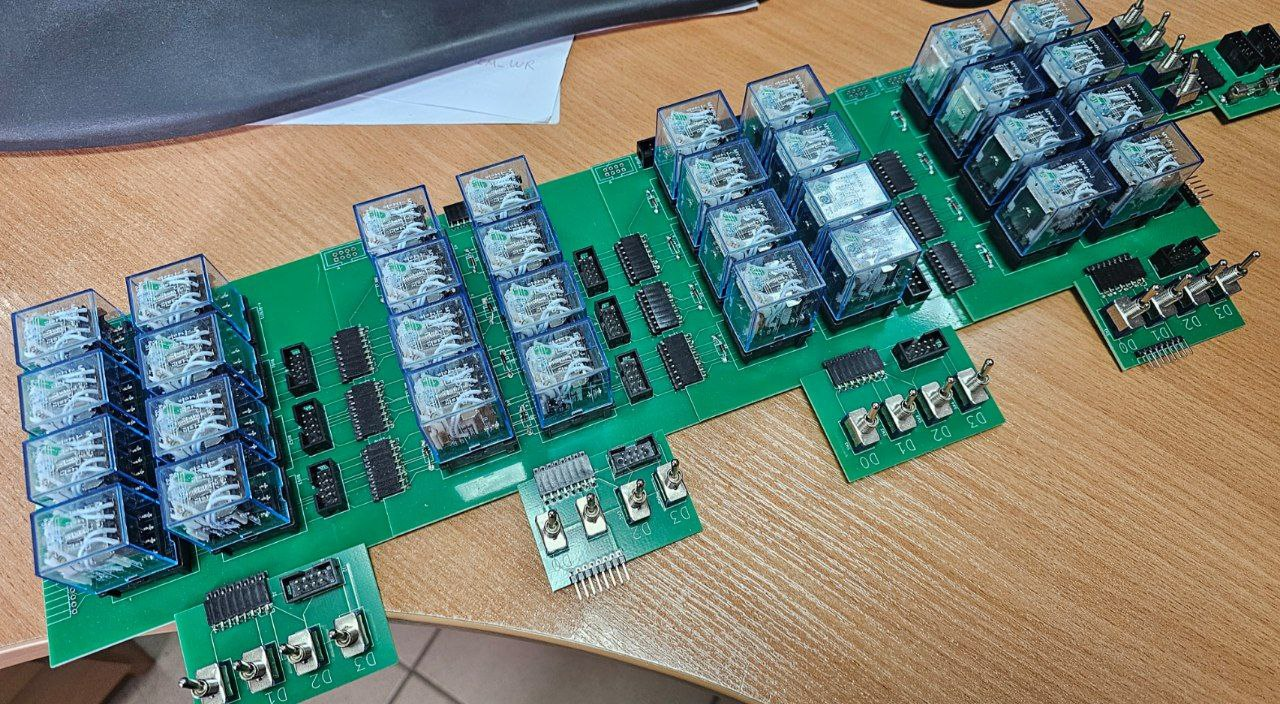
\includegraphics[width=\columnwidth]{photo/register_file.jpg}

Запись в регистры:

\begin{enumerate}
    \item Отключить все управляющие сигналы.
    \item Набрать значение на тумблерах, подключённых к шине данных $1$.
    \item Подключить с помощью тумблера регистр к шине $1$. Убедиться, что в него записалось набранное значение.
    \item Отключить регистр от шины.
    \item Подключить другой регистр к шине $1$. Убедиться, что в него записалось набранное значение.
\end{enumerate}

Копирование значения:

\begin{enumerate}
    \item Отключить все управляющие сигналы.
    \item Подключить регистр с ненулевыми битами к шине $2$.
    \item Подключить пустой регистр к шине $2$. убедиться, что он получил такое же значение, что и в первом регистре.
    \item Отключить все управляющие сигналы.
    \item Аналогично проверить шину $3$.
\end{enumerate}


\section{Унарные логические операции}

Модуль для унарных операций выполняет действия над $4$-битным числом: сдвиг вправо и инверсия битов.

Может каскадироваться для сдвига $8$-битных чисел.

\subsection{Практикум}

На вход модуля унарных операций подключается модуль с тумблерами.
Выходы подключаются к шинам регистра.


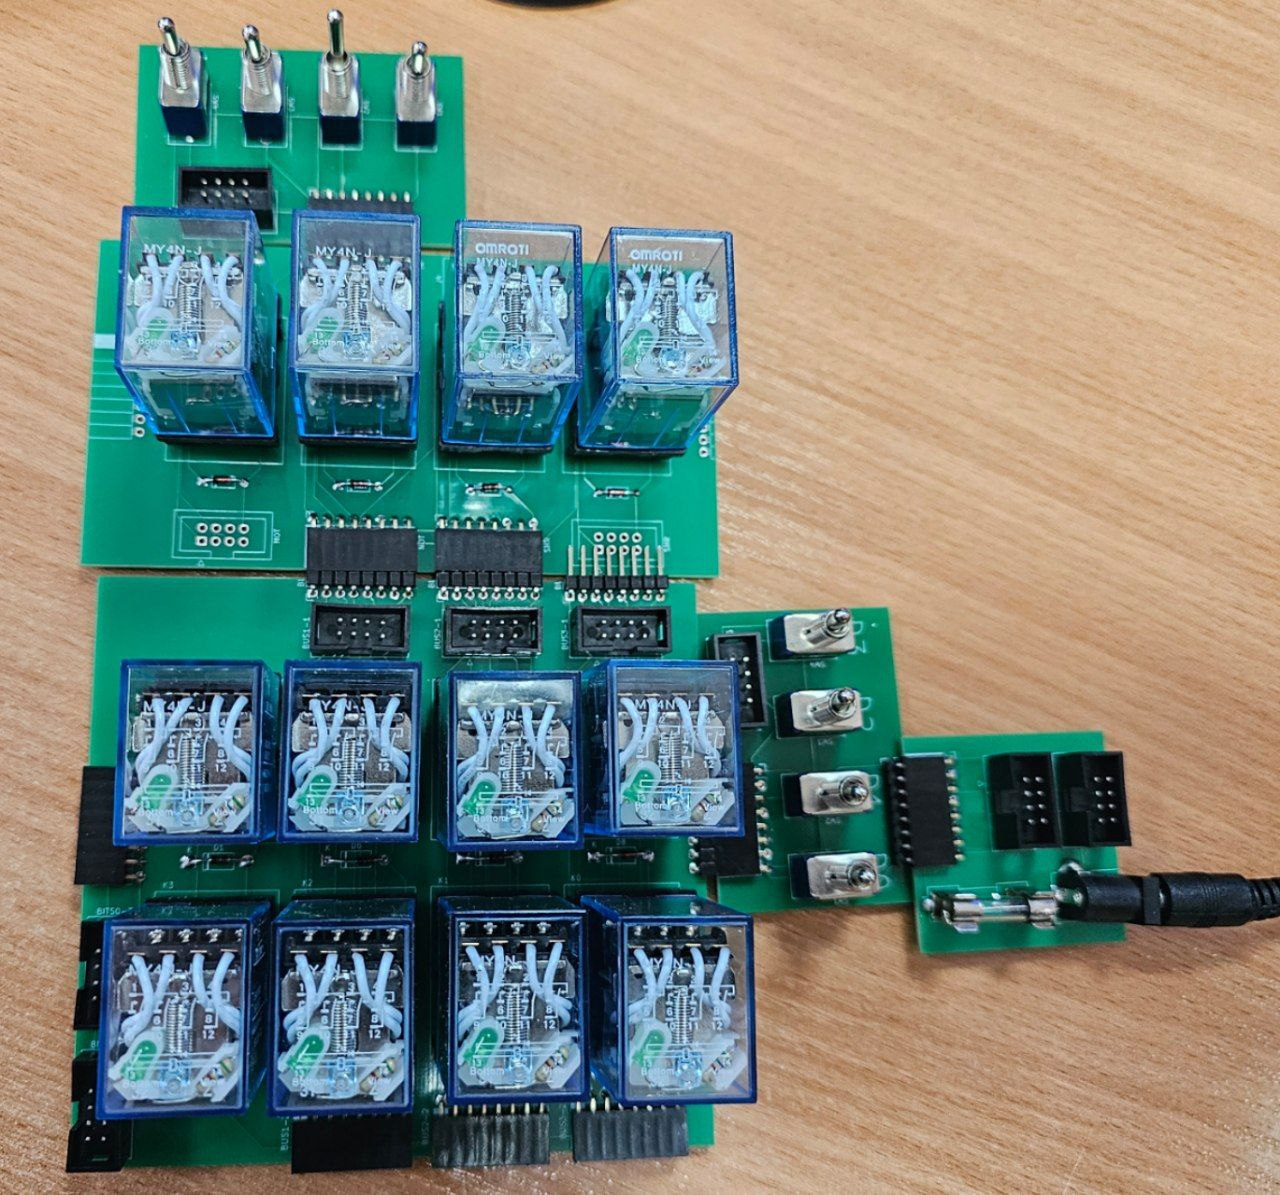
\includegraphics[width=0.5\columnwidth]{photo/unary.jpg}

\begin{enumerate}
    \item Отключить все управляющие сигналы.
    \item Набрать на тумблерах со входными данными значение $1100$.
    \item Подключить выходной регистр к шине $1$. Убедиться, что в него записалось значение $0011$ (инверсия).
    \item Отключить регистр от шины, сбросить его значение.
    \item Подключить выходной регистр к шине $2$. Убедиться, что в него записалось значение $0110$ (сдвиг вправо).
\end{enumerate}

\section{Бинарные логические операции}

Модуль логических операций поддерживает вычисление AND, OR и XOR.
У модуля есть два четырёхбитных входа и три выхода.
Каждый выход отвечает за одну операцию.

\subsection{Практикум}

Ко входам модуля подключаются два модуля с тумблерами, а к выходам --- регистр,
куда будет записываться результат.


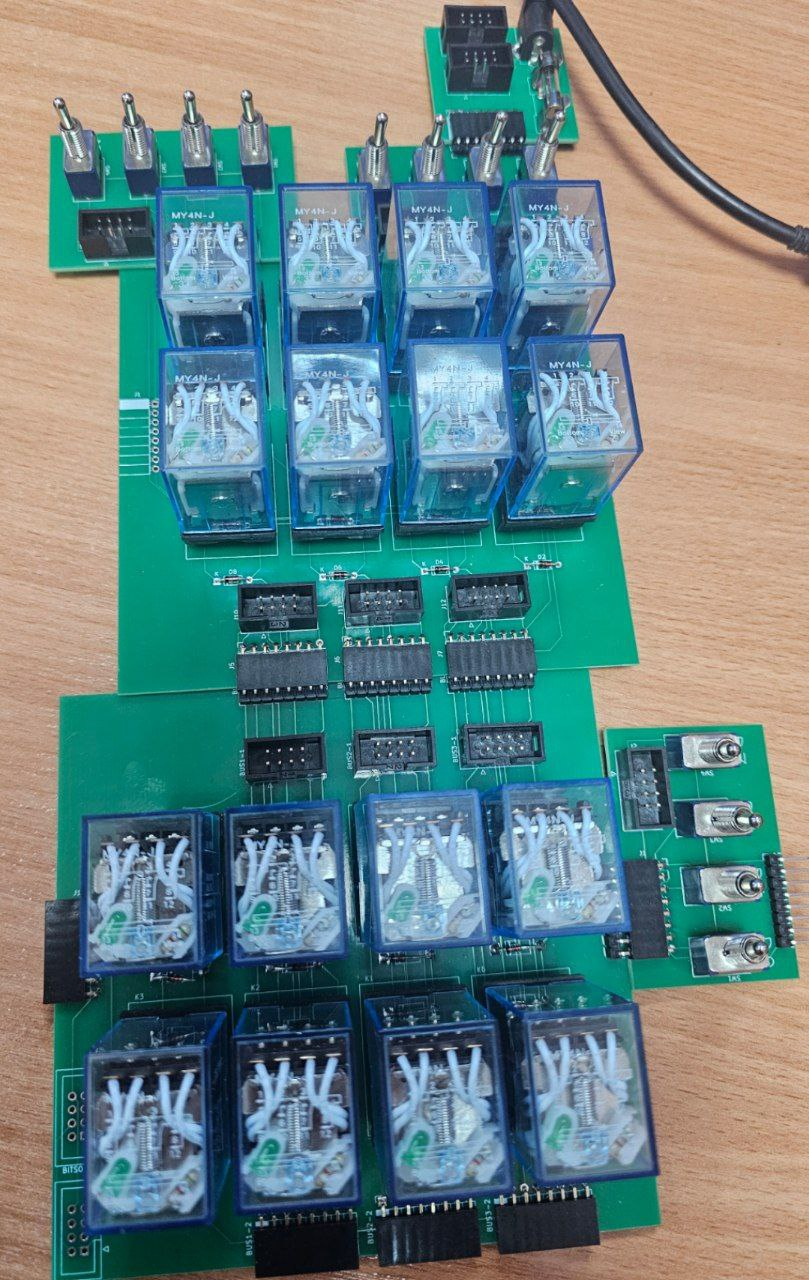
\includegraphics[width=0.5\columnwidth]{photo/logic.jpg}

\begin{enumerate}
    \item Отключить все управляющие сигналы.
    \item Набрать на тумблерах первого операнда значение $1100$.
    \item Набрать на тумблерах второго операнда значение $1010$.
    \item Подключить выходной регистр к шине $1$. Убедиться, что в него записалось значение $1000$ (AND).
    \item Отключить регистр от шины, сбросить его значение.
    \item Подключить выходной регистр к шине $2$. Убедиться, что в него записалось значение $1110$ (OR).
    \item Отключить регистр от шины, сбросить его значение.
    \item Подключить выходной регистр к шине $3$. Убедиться, что в него записалось значение $0110$ (XOR).
\end{enumerate}


\section{Сложение}

Сумматор складывает два четырёхбитных числа, один бит переноса и выдаёт четырёхбитное число и бит переноса.
У модуля есть два четырёхбитный вход и один выход.
Каждый выход отвечает за одну операцию.


\subsection{Практикум}

Ко входам модуля подключаются два модуля с тумблерами, а к выходам --- регистр,
куда будет записываться результат.

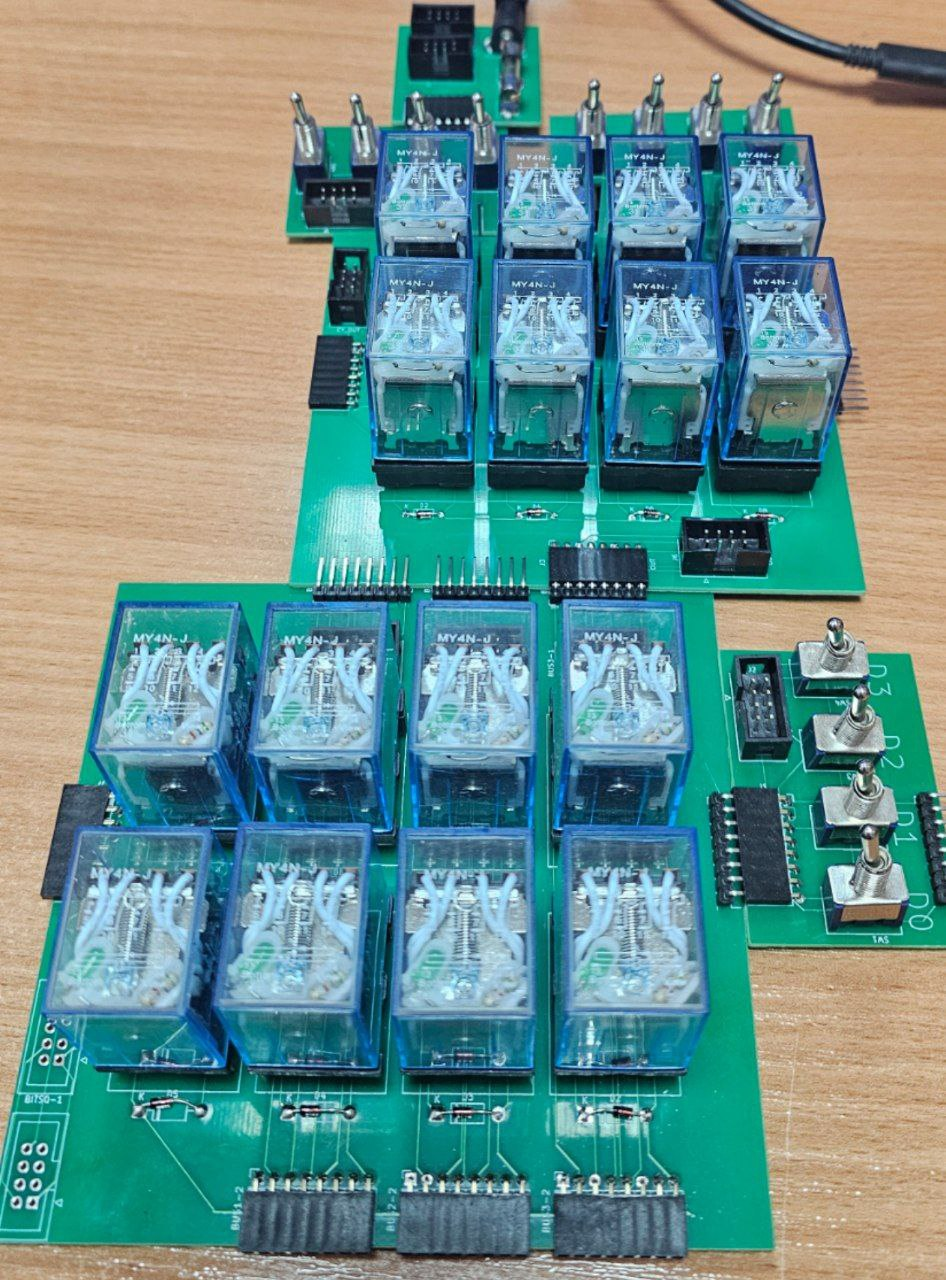
\includegraphics[width=0.5\columnwidth]{photo/adder.jpg}

\begin{enumerate}
    \item Отключить все управляющие сигналы.
    \item Установить перемычку для подачи сигнала на $~CY$.
    \item Набрать на тумблерах первого операнда значение $0011$ (число $3$).
    \item Набрать на тумблерах второго операнда значение $1010$ (число $10$).
    \item Подключить выходной регистр к шине $3$. Убедиться, что в него записалось значение $1101$ (число $13$).
    \item Отключить регистр от шины, сбросить его значение.
    \item Установить перемычку для подачи сигнала на $CY$.
    \item Подключить выходной регистр к шине $3$. Убедиться, что в него записалось значение $1110$ (число $14$).
\end{enumerate}


\section{Вычитание}

\subsection{Вычитание через сложение с дополнительным обратным кодом}

Чтобы вычесть из одного числа другое, можно вычитаемое представить в дополнительном обратном
коде, а затем сложить это число с уменьшаемым.

Число в дополнительном обратном коде получается, если сначала инвертировать биты исходного
числа, а затем прибавить к нему единицу.

Например, для числа $3=0011$ инверсия будет выглядеть, как $1100$, а дополнительный обратный код, как $1101$.

\subsubsection{Практикум}

Собрать схему для сложения.

\begin{enumerate}
    \item Отключить все управляющие сигналы.
    \item Установить перемычку для подачи сигнала на $~CY$.
    \item Набрать на тумблерах первого операнда значение $1010$ (число $10$).
    \item Набрать на тумблерах второго операнда значение $1101$ (число $-3$).
    \item Подключить выходной регистр к шине $3$. Убедиться, что в него записалось значение $0111$ (число $7$).
\end{enumerate}


\subsection{Вычитание с помощью сумматора и инвертора}

Вычитание можно делать с помощью сумматора. Чтобы на входе из операнда получался дополнительный
обратный код, сначала нужно преобразовать его с помощью инвертора, а затем прибавить $1$,
включив вход переноса в сумматоре.

\subsubsection{Практикум}

Собрать схему для сложения, а затем добавить между тумблерами со вторым операндом
инвертор (выход NOT блока унарной логики):

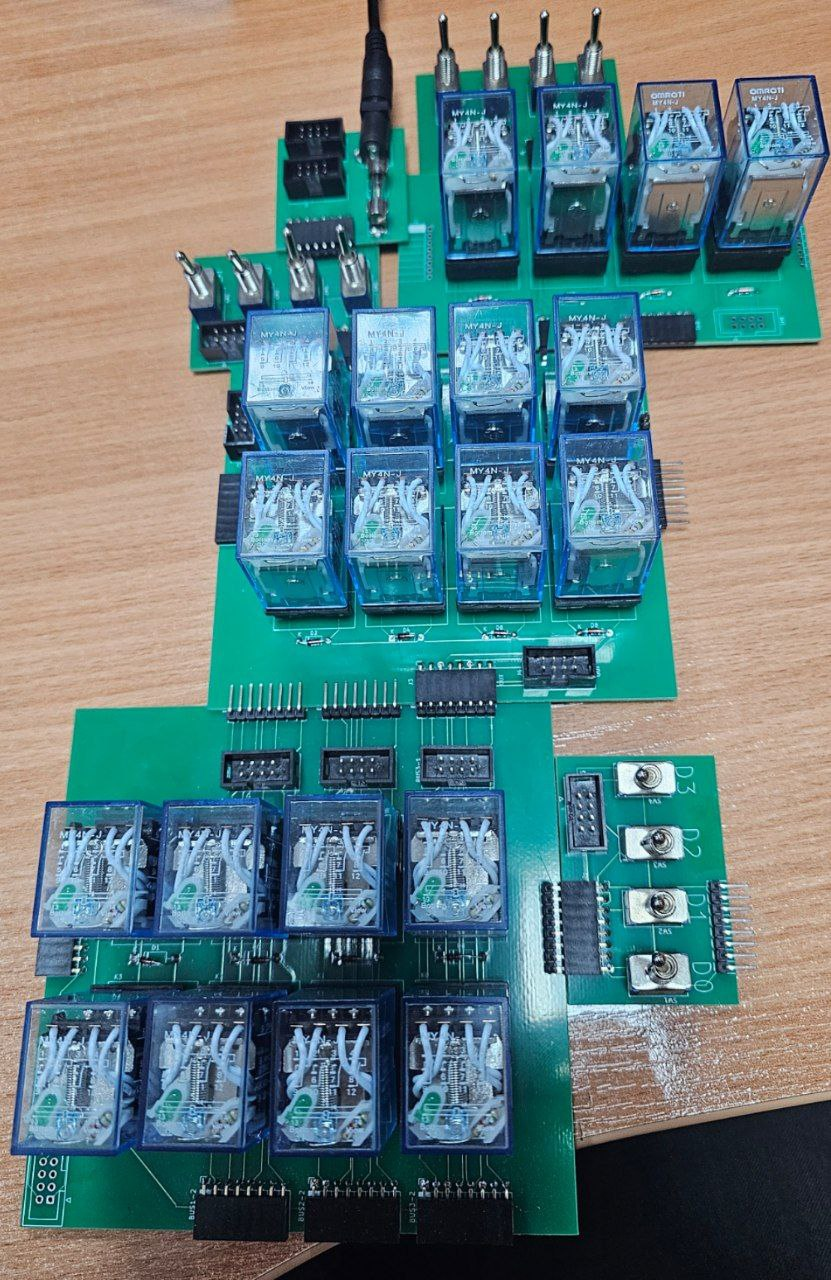
\includegraphics[width=0.5\columnwidth]{photo/subtractor.jpg}

\begin{enumerate}
    \item Отключить все управляющие сигналы.
    \item Установить перемычку для подачи сигнала на $CY$.
    \item Набрать на тумблерах первого операнда значение $1010$ (число $10$).
    \item Набрать на тумблерах второго операнда значение $0011$ (число $3$).
    \item Подключить выходной регистр к шине $3$. Убедиться, что в него записалось значение $0111$ (число $7$).
\end{enumerate}


\section{Целый калькулятор}

Все вычислители можно соединить с одним и тем же регистром, как хранилищем результата, чтобы получить простейший
калькулятор. Доступны следующие операции:
\begin{enumerate}
    \item Инверсия
    \item Сдвиг вправо
    \item Побитовое И
    \item Побитовое ИЛИ
    \item Исключающее ИЛИ
    \item Сложение
    \item Вычитание
\end{enumerate}

\subsubsection{Практикум}

Уже проверенные модули для разных операций соединяются вместе.
Для этого используются несколько мультиплексоров (шинных формирователей)
на платах регистров. На этих платах не установлены реле для хранения
битов. Вместо этого шины подключаются к одному и тому же регистру.
Так в него можно записывать любой из $7$ результатов вычислений.

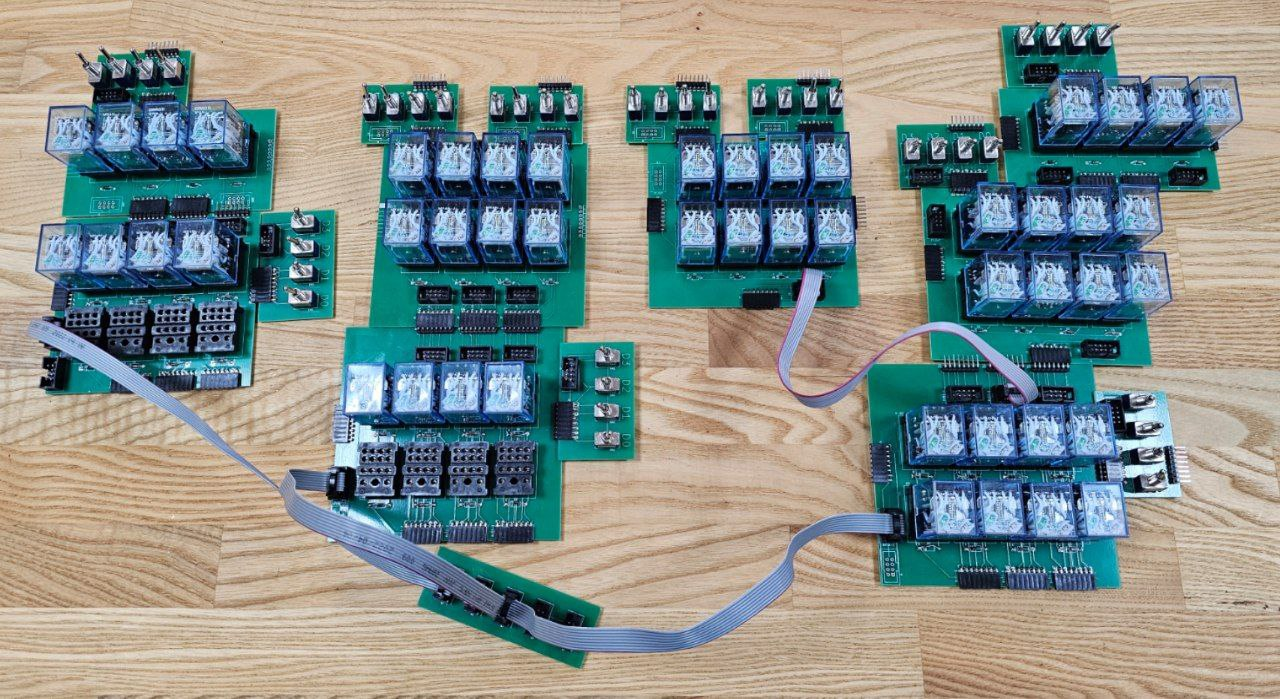
\includegraphics[width=\columnwidth]{photo/calculator.jpg}

Любую из операций можно выполнить так:

\begin{enumerate}
    \item Отключить все управляющие сигналы.
    \item Набрать входные данные для нужной операции.
    \item Подключить выход нужного модуля к регистру тумблером.
    \item Наблюдать результаты вычислений.
    \item Сбросить значение регистра.
\end{enumerate}


\section{Расширение вычислений до восьми бит}

У регистров и вычислительных модулей справа и слева есть разъёмы для расширения разрядности.

Для регистров через эти разъёмы передаются сигналы сброса и подключения к шинам. Поэтому
однин набро тумблеров может использоваться для двух четырёхбитных плат-регистров, если они
соединены в один восьмибитный регистр.

Для вычислительных модулей через боковые разъёмы передаются сигналы переноса (в случае сдвига и сложения).

\subsubsection{Практикум}

Соединить два регистра и два сумматора. Шина $3$ регистров подключается к сумматору.
У правого (младшего) сумматора входящий перенос перемычкой устанавливается в $0$.
У левого (старшего) сумматора перемычка для переноса убирается, потому что
сигнал переноса приходит от младших битов (из правого сумматора).

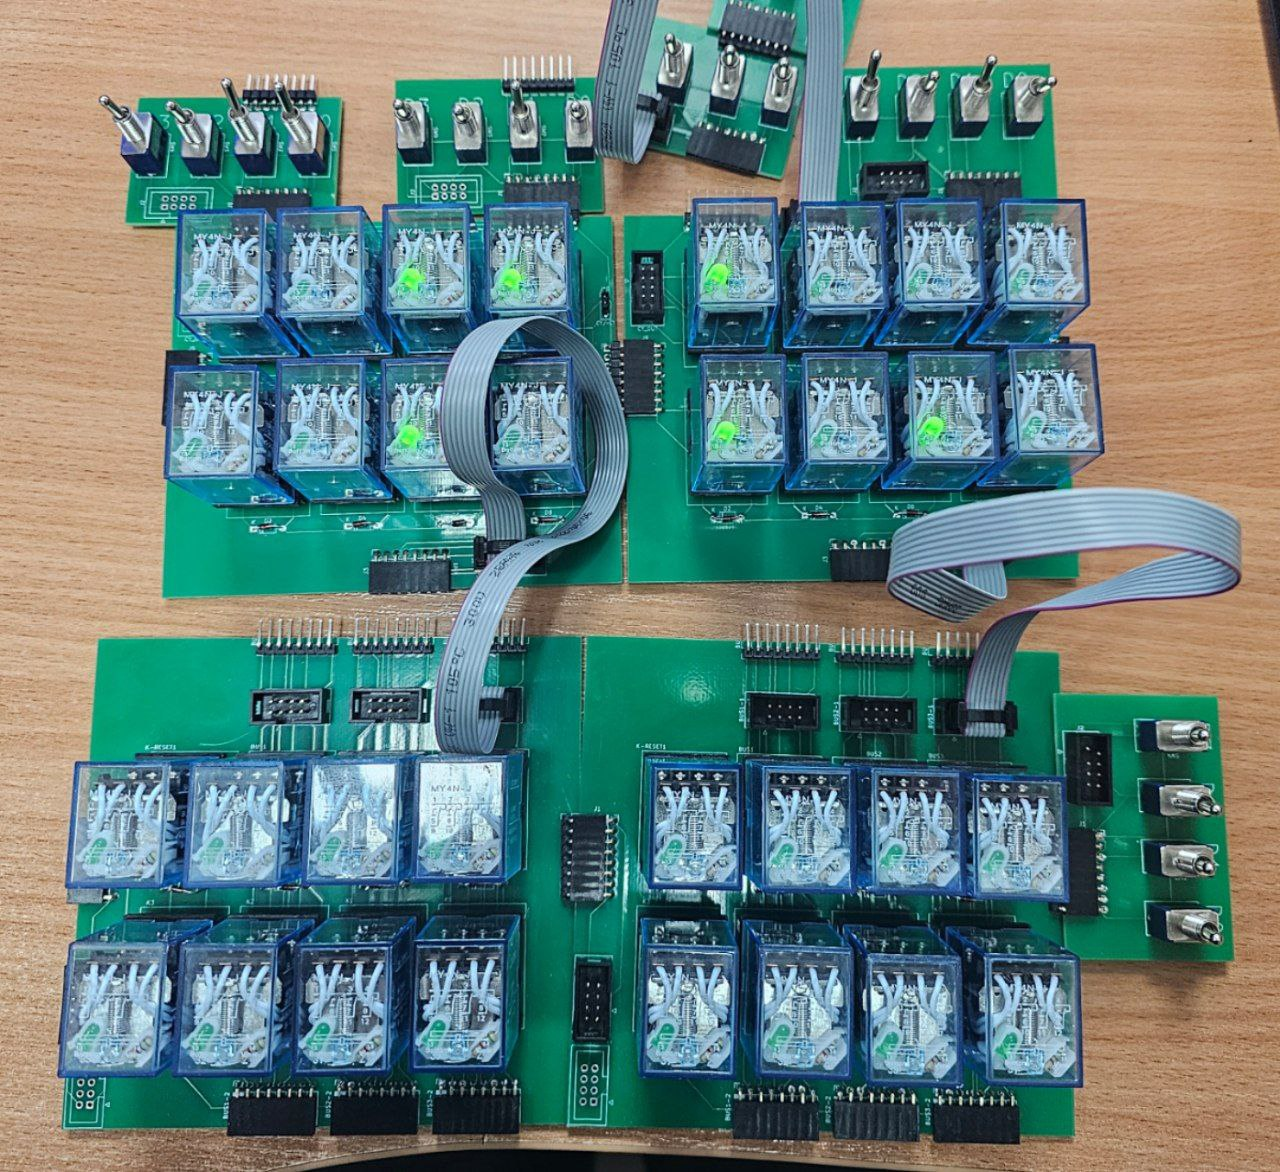
\includegraphics[width=0.5\columnwidth]{photo/8bit.jpg}

\begin{enumerate}
    \item Отключить все управляющие сигналы.
    \item Набрать входные данные $0011 1001$ и $0010 1001$.
    \item Подключить выход сумматора к регистру тумблером $D3$.
    \item Наблюдать результат вычислений $0110 0010$.
\end{enumerate}

\chapter{Элементы компьютера}

\section{Дешифратор}

\section{ПЗУ}

\section{Декодер инструкций}

\chapter{Компьютер}

\end{document}
